% Generated by scripts/question_diversity.py -- do not edit by hand.
\begin{figure*}[t]
\centering
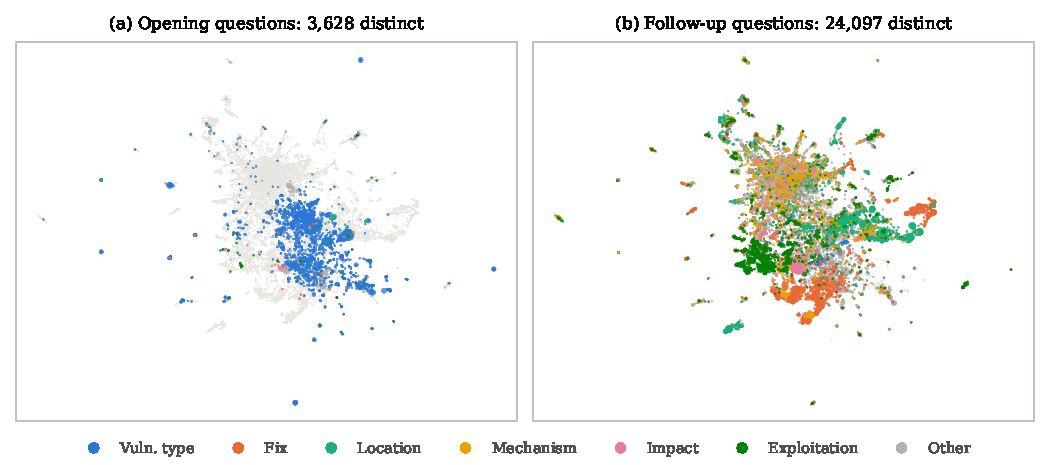
\includegraphics[width=\textwidth]{fig_question_map.pdf}
\caption{Map of the 27,546 distinct questions (sentence embeddings projected with UMAP;
nearby points ask similar things). Colour is the question topic; point area grows with how often a question
occurs. (a)~Opening questions are concentrated: the five most frequent cover 63.8\% of the
26,003 conversations. (b)~Follow-up questions spread over the whole map: 24,097 distinct
questions among 93,115, the five most frequent covering 24.4\%.}
\label{fig:question-map}
\end{figure*}
